\chapter{Electrical}
% Good reference https://www.cougarrobotics.com/wp-content/uploads/2016/11/Using-Sensors-2018.pptx.pdf

\section{Power Electronics}

\subsection{Batteries}
% Internal resistance, chemistries, ratings
\subsection{Breakers}
% Match gague to breakers
\subsection{Wires}
% Minimize run lengths
% Voltage drop over wires

\subsection{Terminals and Connectors}
% Encyclopedia of the different types

\section{Sensors}

\subsection{On/Off Position Sensors}
\begin{figure}[H]
\begin{subfigure}[b]{.31\linewidth}
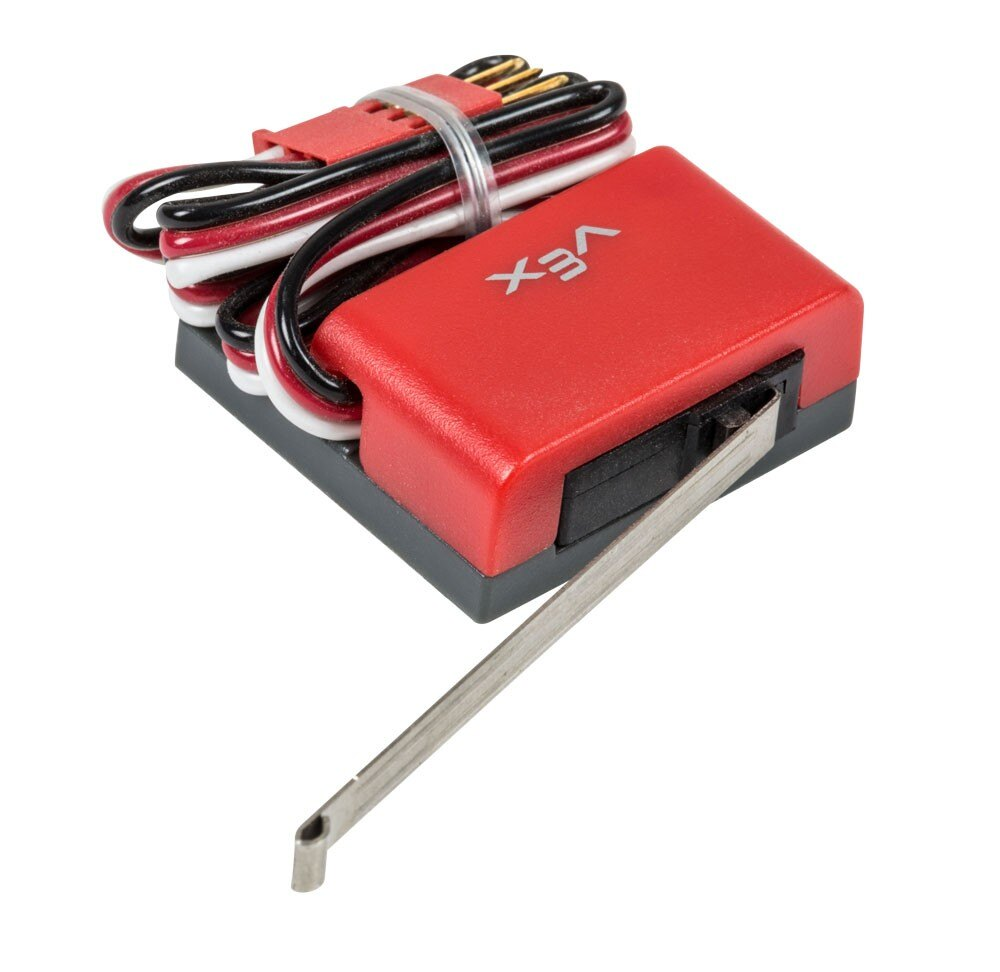
\includegraphics[width=.8\textwidth]{imgs/sensor_limitswitch.jpeg}
\subcaption{Limit Switch}
\end{subfigure}\begin{subfigure}[b]{.31\linewidth}
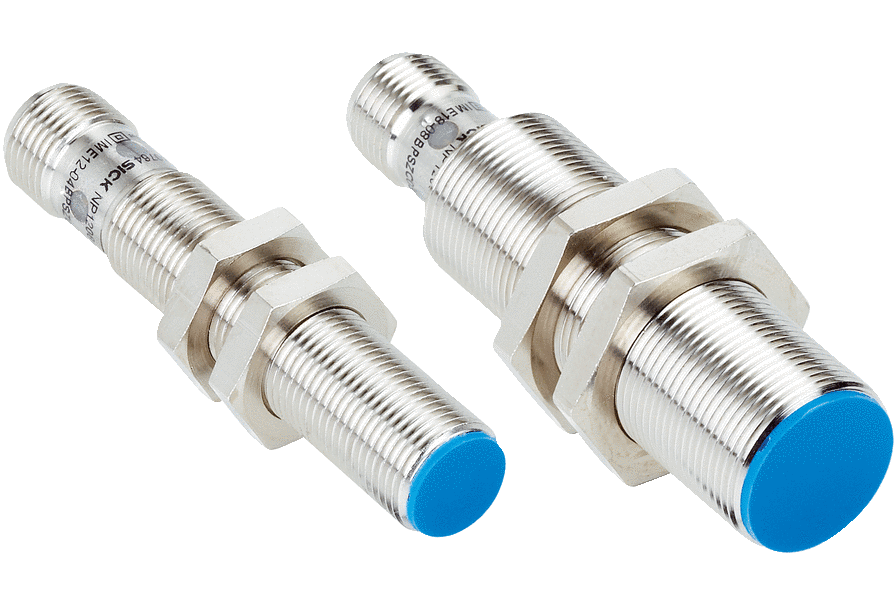
\includegraphics[width=.8\textwidth]{imgs/sensor_indprox.png}
\subcaption{Inductive Proximity Switch}
\end{subfigure}\begin{subfigure}[b]{.31\linewidth}
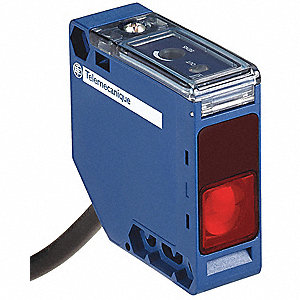
\includegraphics[width=.8\textwidth]{imgs/sensor_beambreak.jpeg}
\subcaption{IR Photoeye}
\end{subfigure}
\end{figure}

\begin{asparaenum}[a)]
\item \textit{Limit switches} are basic switches. They mechanically switch power between different positions- so do not require power to operate them (just signal).
\item \textit{Inductive proximity switches} send out a magnetic field and detect interference in this field caused by metallic objects (\textit{ferrous} metals usually work best). This allows them to sense if an object is in position without risking dangerous mechanical contact. They require appropriate power to operate (refer to their datasheet for requirements). These sensors come in different packages, although the screw-body style shown is the most common. They are also rated by their minimum and maximum sensing distances.
\item \textit{IR photoeyes} emit infrared radiation and measure how much is reflected back. This allows any object to be detected if it is within the sensing range. They require power to operate (refer to their datasheet for requirements). \item \textit{Beam breaks} emit infrared lasers and collect them on the opposite side. If an object blocks the path, the beam is broken, causing a change in signal. 
\end{asparaenum}

Sensors can be wired in various ways.

\begin{figure}[H]
\begin{subfigure}[b]{.4\linewidth}
\begin{circuitikz}[american voltages] \draw
  (0,0) node[ground]{} to [R] (0,2)
  to [push button, *-o] (0,4) node[left]{$V$};
  \draw (+2,2) node[below]{To input} to [short] (0,2);
\end{circuitikz}
\subcaption{Pull-Down Wiring}
\end{subfigure}\begin{subfigure}[b]{.4\linewidth}
\begin{circuitikz}[american voltages] \draw
  (0,0) node[ground]{} to [push button] (0,2)
  to [R, *-o] (0,4) node[left]{$V$};
  \draw (+2,2) node[below]{To input} to [short] (0,2);
\end{circuitikz}
\subcaption{Pull-Up Wiring}
\end{subfigure}

\begin{subfigure}[b]{.47\linewidth}
\begin{circuitikz}[american voltages]

    \fill[gray] (-1,1)--(-3,1)--(-3,3)--(-1,3)--cycle;
    \draw[black] (-1,1)--(-3,1)--(-3,3)--(-1,3)--cycle;

    \node[black] at (-2,2){NPN Sensor} ;

  \draw (1.5,4) node[left]{$V$} to [R, o-*] (1.5,2);
  \draw (-1,2) -- (2,2) node[below]{To input};
  \draw (-1,1.5) -- (0,1.5) -- (0,0) node[ground]{};
  \draw (-1,2.5) -- (0,2.5) to [short, -o] (0,4) node[left]{$V$};
\end{circuitikz}
\subcaption{NPN Sensor Wiring}
\end{subfigure}\begin{subfigure}[b]{.47\linewidth}
\begin{circuitikz}[american voltages]

    \fill[gray] (-1,1)--(-3,1)--(-3,3)--(-1,3)--cycle;
    \draw[black] (-1,1)--(-3,1)--(-3,3)--(-1,3)--cycle;

    \node[black] at (-2,2){PNP Sensor} ;

  \draw (1.5,0) node[ground]{} to [R, -*] (1.5,2);1
  \draw (-1,2) -- (2,2) node[above]{To input};
  \draw (-1,1.5) -- (0,1.5) -- (0,0) node[ground]{};
  \draw (-1,2.5) -- (0,2.5) to [short, -o] (0,4) node[left]{$V$};
\end{circuitikz}
\subcaption{PNP Sensor Wiring}
\end{subfigure}
\end{figure}

\begin{asparaenum}[a)]
\item \textit{Pull down resistors} make the inputs of a microprocessor rest naturally at ground level. When the connected switch is closed, the resistance of the switch is much much less than the pulldown resistor, so the voltage of the input will rise to the logic voltage. The resistor is sized so as not to consume too much current (usually R = 5 to 20 k\Omega). A microprocessor may have such a resistor built-in to the circuitry, although the resistor may need to be enabled.
\item \textit{Pull up resistors} work on the same principle as pull down resistors but with reversed voltages. On the RoboRIO, 2.2 k\Omega pull-up resistors are on all DIO pins when in input mode.
\item \textit{NPN} and \textit{PNP} sensors are to be wired as shown. You may note that the wiring looks the same as for a pull-up or pull-down; match the type of pulling resistor in your microprocessor to the type of sensor you intend to use, otherwise external pulling resistors may be necessary.
\end{asparaenum}



% Wiring schemes (pull up vs pull down)

\subsection{Variable Position Sensors}
\begin{figure}[H]
\begin{subfigure}[b]{.33\linewidth}
%\includegraphics[height=2.1in]{imgs/sensor_encoder.png}
\subcaption{Encoder}
\end{subfigure}\begin{subfigure}[b]{.33\linewidth}
%\includegraphics[height=2.1in]{imgs/potentiometer.png}
\subcaption{Potentiometer}
\end{subfigure}\begin{subfigure}[b]{.33\linewidth}
%\includegraphics[height=2.1in]{imgs/sensor_lvdt.png}
\subcaption{LVDT}
\end{subfigure}
\end{figure}

\begin{asparaenum}[a)]
\item \textit{Encoders} use rotating discs with multiple on/off positions in them to determine position. The on/off mechanism could be optical, magnetic, or something else entirely. A microprocessor running fast enough can watch the waveform produced by the encoder and determine how much the position has changed. Some encoders have builtin microprocessors, which can feed back more complex signals, while others may simply feed back \textit{quadrature} data from the two channels that are monitored.
\item \textit{Potentiometers} have a resistive element, with the moving wiper making contact somewhere in the middle of it. When the wiper moves, the resistance between the wiper and the ends changes, which allows the voltage to be read. These are inherently absolute sensors- power cycling does not affect the resistance values. \textit{Multi-turn} potentiometers allow the shaft to be rotated multiple times by running the wiper through a helical spiral. Linear potentiometers also exist- they often come in a piston-style package that can be mounted with rod ends.
\item \textit{Linear Variable Differential Transformers (LVDTs)} use multiple magnetic fields and measurements to determine position. They are quite expensive, but can be used in harsh environments with high accuracies. Rotational equivalents (RVDTs) also exist.
\end{asparaenum}

\subsection{Rangefinding}
\begin{asparaenum}[a)]
\item \textit{Ultrasonic sensors} send out high-pitched sound waves and measure how long it takes for them to return. These can be finnicky, and do not work to detect objects that absorb, rather than reflect sound.
\item \textit{Time of flight} sensors work on the same principle as ultrasonic sensors, but with light. Light travels much, much faster- so these devices are more sophisticated and expensive.
\item \textit{LIDAR} systems employ a moving time of flight sensor to build a 3D map of the surroundings.
\item \textit{Computer Vision (CV)} can be used to pick up targets visually and determine their distance and relative position. It's particularly easy when the targets are a specialized color and shape that is distinct from everything else. CV systems can operate on even the simplest of hardware such as a smartphone, but the latency and image quality may suffer. Specialized sensors exist to improve the key performance parameters when using a camera in a real-time system.
\end{asparaenum}

% Don't go too in-depth on these; just talk about pros/cons
\subsection{IMUs}
\begin{asparaenum}[a)]
\item \textit{Gyroscopes} measure the rate of rotational acceleration. They can be used to find rotational velocity and position by performing numeric integration with a computer. As the rotational acceleration/velocity on a rigid body is constant, it does not matter where they are mounted so long as it is of sufficient rigidity and vibration isolation.
\item \textit{Accelerometers} measure linear acceleration. They can be used to find linear velocity and position by performing numeric integration with a computer.
\item \textit{Magnetometers} or \textit{digital compasses} pick up magnetic fields (such as the earth's). This allows them to determine absolute orientation, although magnetic fields can be greatly disturbed by metallic structures and buildings.
\item \textit{Integrated Motion Units} combine several of these sensors into one system, complete with an onboard microprocessor to perform aforementioned numerical integration. This dedicated processing allows them to acheive high integration accuracy.
\end{asparaenum}


\section{Communication Protocols}

\subsection{Dumb signals} % High/low, PWM

\begin{asparaenum}[a)]
\item Simple high and low signals can convey whether something is active or inactive at a particular point in time.
\item Analog signals can convey a particular variable value rather than a high or low. However, they require complex circuits to encode and decode from digital devices
\item \textit{Pulse-width modulation (PWM)} allows for the unidirectional trasmittal of variables over one signal wire without the need for analog circuitry. A square wave of fixed \textit{frequency} is generated and the variable to be sent is encoded in the \textit{pulse width} or \textit{duty cycle}. Typical "servo style" PWM uses a frequency of 50 Hz (or a period of 20 ms), with a pulse width of 1 ms corresponding to the minimum value (full reverse, or 0 degrees), and 2 ms corresponding to the maximum value (full forwards, or 180 degrees). This is a reasonably safe signal to send safety critical functions on as any interruptions to the signal would result in clearly invalid data.
\end{asparaenum}

\subsection{Serial links} % RS232, USB, UART, TTL

Serial encoding of data takes a binary signal and serializes it. For example, the ASCII character `A' is represented in binary as 01000001. So, one device would send a low signal, then a high signal, followed by five low signals, and a final high signal in order to transmit an `A'. It isn't quite this simple, though.

To begin with, data is not always going to be transmitted over the line. The line will be a constant value before the data to be transmitted is sent. The sending device must first send a \textit{start bit} to denote the beginning of a transmission. Additionally, a \textit{stop bit} may be sent to denote the end of the transmission.

\begin{asparaenum}[a)]
\item Serial 
\end{asparaenum}

\subsection{Bus/network signals} % I2C, SPI, CAN, Ethernet

